%
% $Id$
%
\documentclass{article}
\usepackage{epsfig}
\usepackage{rotating}
% \usepackage{subfigure}
% \usepackage{vcode}
\usepackage{xspace}
% \usepackage{gloss}

% Change paragraph typesetting; eliminate indenting and add more space between
% paragraphs. 2/15/2000 jhrg
\setlength{\parindent}{0em}     % Amount of indentation
\addtolength{\parskip}{1ex}     % Vertical separation

% Sample macros including a URL which can be hyphenated. 
\newcommand{\httpd}{\texttt{httpd}\xspace}
\newcommand{\Cpp}{\rm {\small C}\raise.5ex\hbox{\footnotesize ++}\xspace}
\newcommand{\dap}{\rm {\small DAP}\raise.5ex\hbox{\footnotesize ++}\xspace}
\newcommand{\maewesturl}{http://maewest.gso.uri.edu/\-cgi-bin/\-nph-dsp/\-htn\_sst\_decloud/\-1992/\-i92098065016.htn\_d.Z\xspace}

\begin{document}

\title{DAP Description}
\author{James Gallagher\thanks{jgallagher@gso.uri.edu}
  \and Dan Holloway\thanks{d.holloway@gso.uri.edu}}
\date{\today \\ $Revision$ }

\maketitle
\tableofcontents

\section{Representing Information in a Dataset}
\label{sec:representation}

\begin{itemize}
\item Represent datasets as a collection of variables, each of which has a
  name, datatype and its own collection of attributes.

\item Variable names are identifiers.
  
\item Datatypes are similar to those found in a programming language. The
  supported primitive types are: 
  \begin{enumerate}
  \item Byte
  \item Int (16 and 32 bit, both signed and unsigned)
  \item Float (32 and 64 bit)
  \item String
  \item URL
  \end{enumerate}
  Available constructor types are:
  \begin{enumerate}
  \item Array
  \item List 
  \item Structure
  \item Sequence 
  \item Grid
  \end{enumerate}
  There are some limits placed on what the constructor types may contain.
  
\item Each variable has a collection of attributes. Each attribute has a
  name, type and value(s). For attributes, all the primitive types are
  supported plus undimensioned vectors and structures (although the later is
  called `container' in the documentation).

\item The DAP is a stateless protocol.
\end{itemize}

\begin{quote}
For more inforamtion about using the \dap class library, see the DODS
Programmer's Guide (http://unidata.ucar.edu/packages/dods/).
\end{quote}

\section{How the DAP Answers a Request}
\label{sec:answer}

The DAP returns information using one of three objects: DDS, DAS and DataDDS.
\begin{itemize}
\item The DDS is a container which holds variables.\footnote{We could have
  implemented this using the Structure class, but didn't.} When a DODS server
is asked which variables are in a dataset, it returns an instance of this
object.
  
\item The DAS is a container which holds each variable's attributes. When a
  DODS server is asked about the attributes associated with each variable in
  a dataset, it returns this object.\footnote{The DAS and DDS are separate
    containers mostly for historical (hysterical?) reasons. It would be
    straightforward to merge this information into the DDS, but the
    separation simpilifies the servers somewhat and it's easy to merge the
    DAS and DDS on the client side.}

\item The DataDDS is a DDS object whose component variables can contain data.
  When a DODS server is asked to return data, it does so using this object.
  There's very little difference between a DDS and a DataDDS object. However,
  servers use the two objects for different purposes, so the distinction is
  useful.
\end{itemize}

\section{Moving Binary Objects from Server to Client}
\label{sec:binary}

\begin{itemize}
  
\item In DODS, clients get objects from a remote source and operate on them
  locally.
  
\item All three objects are transformed from a binary representation to a
  persistent representation before being transmitted.
  
\item Once recieved, objects are reconstituted so that clients can use them
  just like local objects (because they are local objects).
  
\item A class called Connect encapsulates the actual process of requesting an
  object from a server. Section~\ref{sec:client} shows how an instance of
  Connect is used to get object from a server.
  
\item The persistent represenation for a DDS or DAS object is as structured
  text\footnote{No, not XML, but it could be with very little work. \ldots
    like so many other things \ldots} wrapped in a MIME document whose
  Content-Type is text/plain. Thus the persistent represetations of these
  objects can be viewed in a web browser.
  
\item The \dap class library contains parsers which read these documents and
  generates their binary representations. In Section~\ref{sec:variables} the
  classes used to represent these variables are described. Since the classes
  are abstract, virtual constructors (or factory methods) are used by the
  parsers to instantiate concrete subclasses defined for a particular
  application. The concrete classes must define the virtual constructors.
  
\item The DataDDS object is a multipart MIME document which holds both a DDS
  and set of values encoded in XDR. The DDS object lists the variables
  in the order their values appear in the second part of the document.
  
\item Since the DataDDS is a binary MIME document, web browsers will only
  offer to save the response to a file. This is the one object that cannot be
  visualized in some way by a web browser.

\end{itemize}

\section{Representing Variables in the DAP}
\label{sec:variables}

See Figures~\ref{fig:basetype}~and~\ref{fig:subclasses}.

\begin{itemize}
\item Variables are represented using children of the class \emph{BaseType}.
  
\item There is a subclass for each datatype which the DAP can use to
  represent variables in a dataset. Each of these classes are abstract.
  
\item Figure~\ref{fig:subclasses} shows one way to use the datatype classes
  in a DODS client. The concrete classes NCWriteByte, \ldots, inherit from
  both \emph{Byte} and \emph{NCWriter}. Look at the source code in
  \texttt{DODS/\-src/\-tools/\-ascii} and
  \texttt{DODS/\-src/\-clients/\-ml-cmdln} for some sample clients.
  
\item Both clients and servers that use the DAP datatype classes must
  provide a factory method\footnote{Or a virtual constructor, depending on
    who you read and how specific you want to be about the words \ldots} so
  that the software which creates the objects (e.g., when decoding a response
  from a server) will create instances of the concrete classes.
\end{itemize}

\begin{sidewaysfigure}[h]
\begin{center}
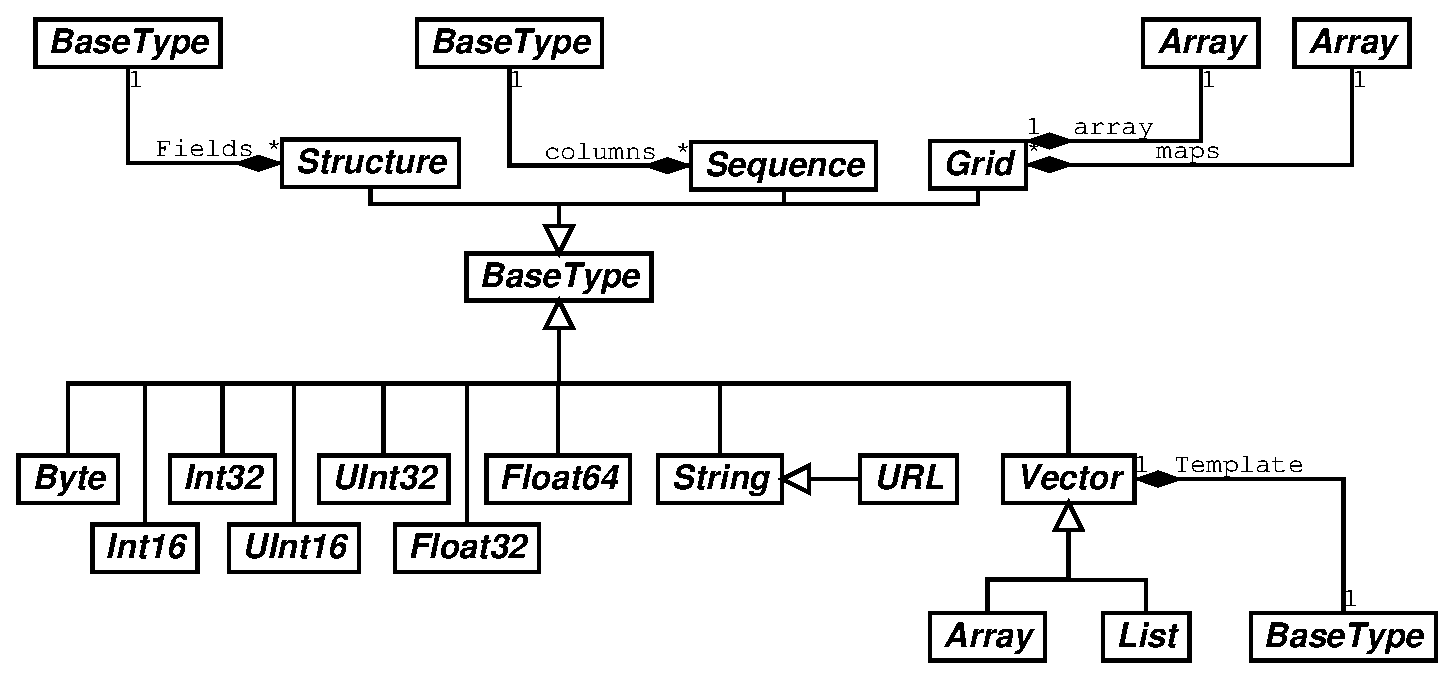
\epsfig{file=dods-datatype-class.eps,width=7.5in}
\caption{Datatype classes. This uses the Composite pattern described by
  Gamma, \textit{et al.}}
\label{fig:basetype}
\end{center}
\end{sidewaysfigure}

\begin{sidewaysfigure}[h]
\begin{center}
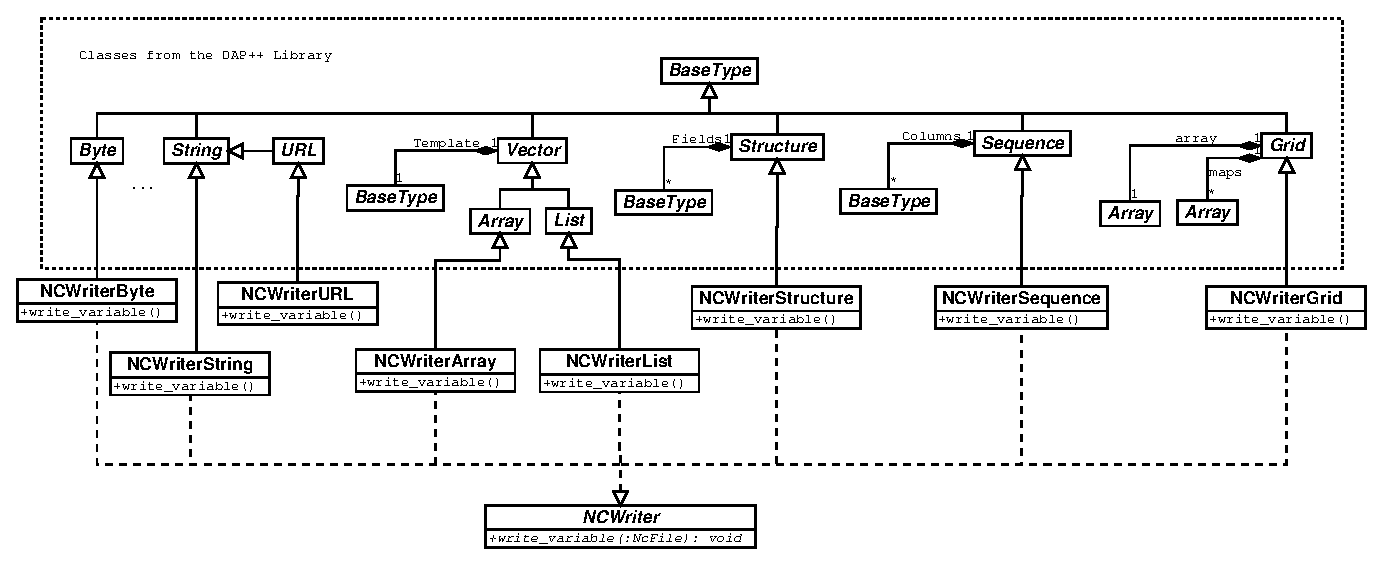
\epsfig{file=file-format-writer.eps,width=7.5in}
\caption{Example use of the datatype classes. This shows the classes
  specialized to read data and write out the values in a NetCDF file. This is
  from a design that has not yet (11/6/2000 jhrg) been fully implemented but
  is very similar to other designs we've used in the past.}
\label{fig:subclasses}
\end{center}
\end{sidewaysfigure}

\section{Representing Metadata}
\label{sec:metadata}

See Figures~\ref{fig:attributes}~and~\ref{fig:interface}.

\begin{itemize}
\item Each variable has an associated `Attribute Table' which holds
  information beyond the name, datatype and value of the variable.
  
\item A variable may have no attributes or it may have many.
  
\item A DAS object is a container for attribute table (AttrTable) objects. An
  attribute table is a container for attribtues. An attribute is either a
  name-type-value tuple or it is a name and attribute table pair. See
  Figure~\ref{fig:attributes}.
  
\item Values are limited to the primitive datatypes and undimensioned
  vectors.
  
\item Named attribute tables are effectively structures for attributes.
  
\item Unlike variables, attributes are not abstract and an attribute tuple
  always has a value (When a variable is part of a DDS it has no value; only
  variables in a DataDDS can have values).
  
\item In essence, the DDS is also metadata. The information in the DDS is
  required to represent the values in a computer. The information in a DAS is
  desireable since it makes the information useful to a person or an analysis
  algorithm.
  
\item It is convenient to combine information in the DDS and DAS for many
  clients.  This is simple to do by adding an instance of AttrTable to the
  concrete datatype classes and providing an accessor method for that
  attribtue table via an interface. A simple algorithm can be used to move
  AttrTable objects from the DAS to the DDS. See Figure~\ref{fig:interface}
  and \texttt{DODS/\-src/\-clients/\-ml-cmdln/}.

\item DODS also supports `Global' attributes. These are attibutes which are
  not associated with any of the dataset's variable. Instead they apply to
  the whole dataset. A dataset may have any number of global attribute
  containers.

\item Adding extra attribute containers is a good way to include several
  different sets of metadata with a single dtatset. This provides a way to
  support several metadata `namespaces' at once.
\end{itemize}

\begin{figure}[h]
\begin{center}
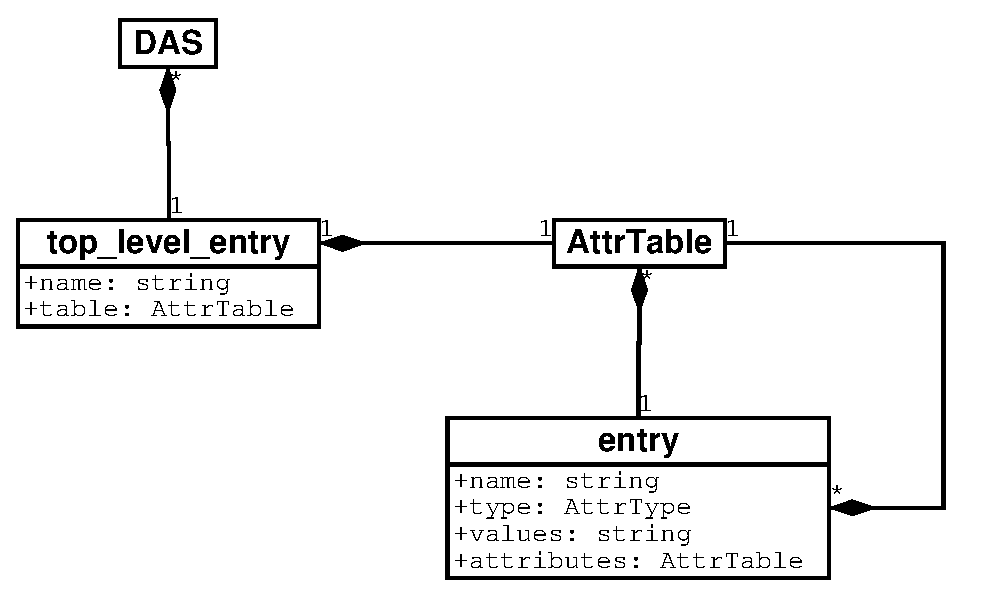
\epsfig{file=attributes.eps,width=4.5in}
\caption{Classes used to hold attribute inforamtion.}
\label{fig:attributes}
\end{center}
\end{figure}

\begin{sidewaysfigure}[h]
\begin{center}
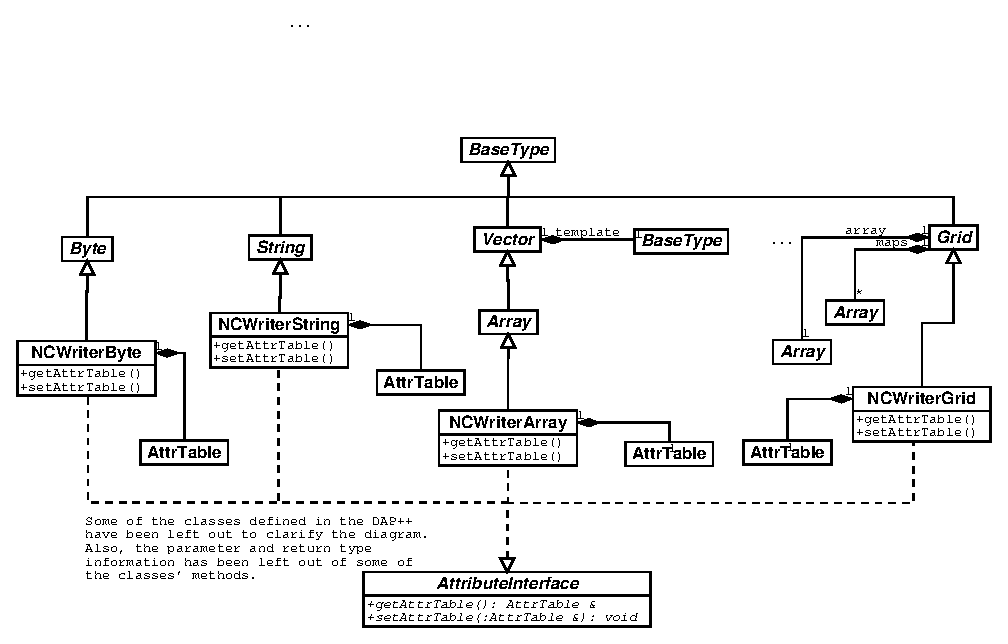
\epsfig{file=file-format-with-attrs.eps,width=7.5in}
\caption{Using an interface to combine information from the DAS and DDS
  objects.} 
\label{fig:interface}
\end{center}
\end{sidewaysfigure}

\section{Using the DAP in a Client}
\label{sec:client}

See Figure~\ref{fig:client}.

\begin{itemize}
\item A DODS client instantiates Connect to establish a virtual connection
  with a server.
  
\item The instance of Connect (aConnect in Figure~\ref{fig:client}) is then
  used to request objects from the server.
  
\item The client \texttt{geturl} is very simple. Its source code can be found
  in \texttt{DODS/\-src/\-dap/\-geturl.cc}.
\end{itemize}

\begin{sidewaysfigure}[h]
\begin{center}
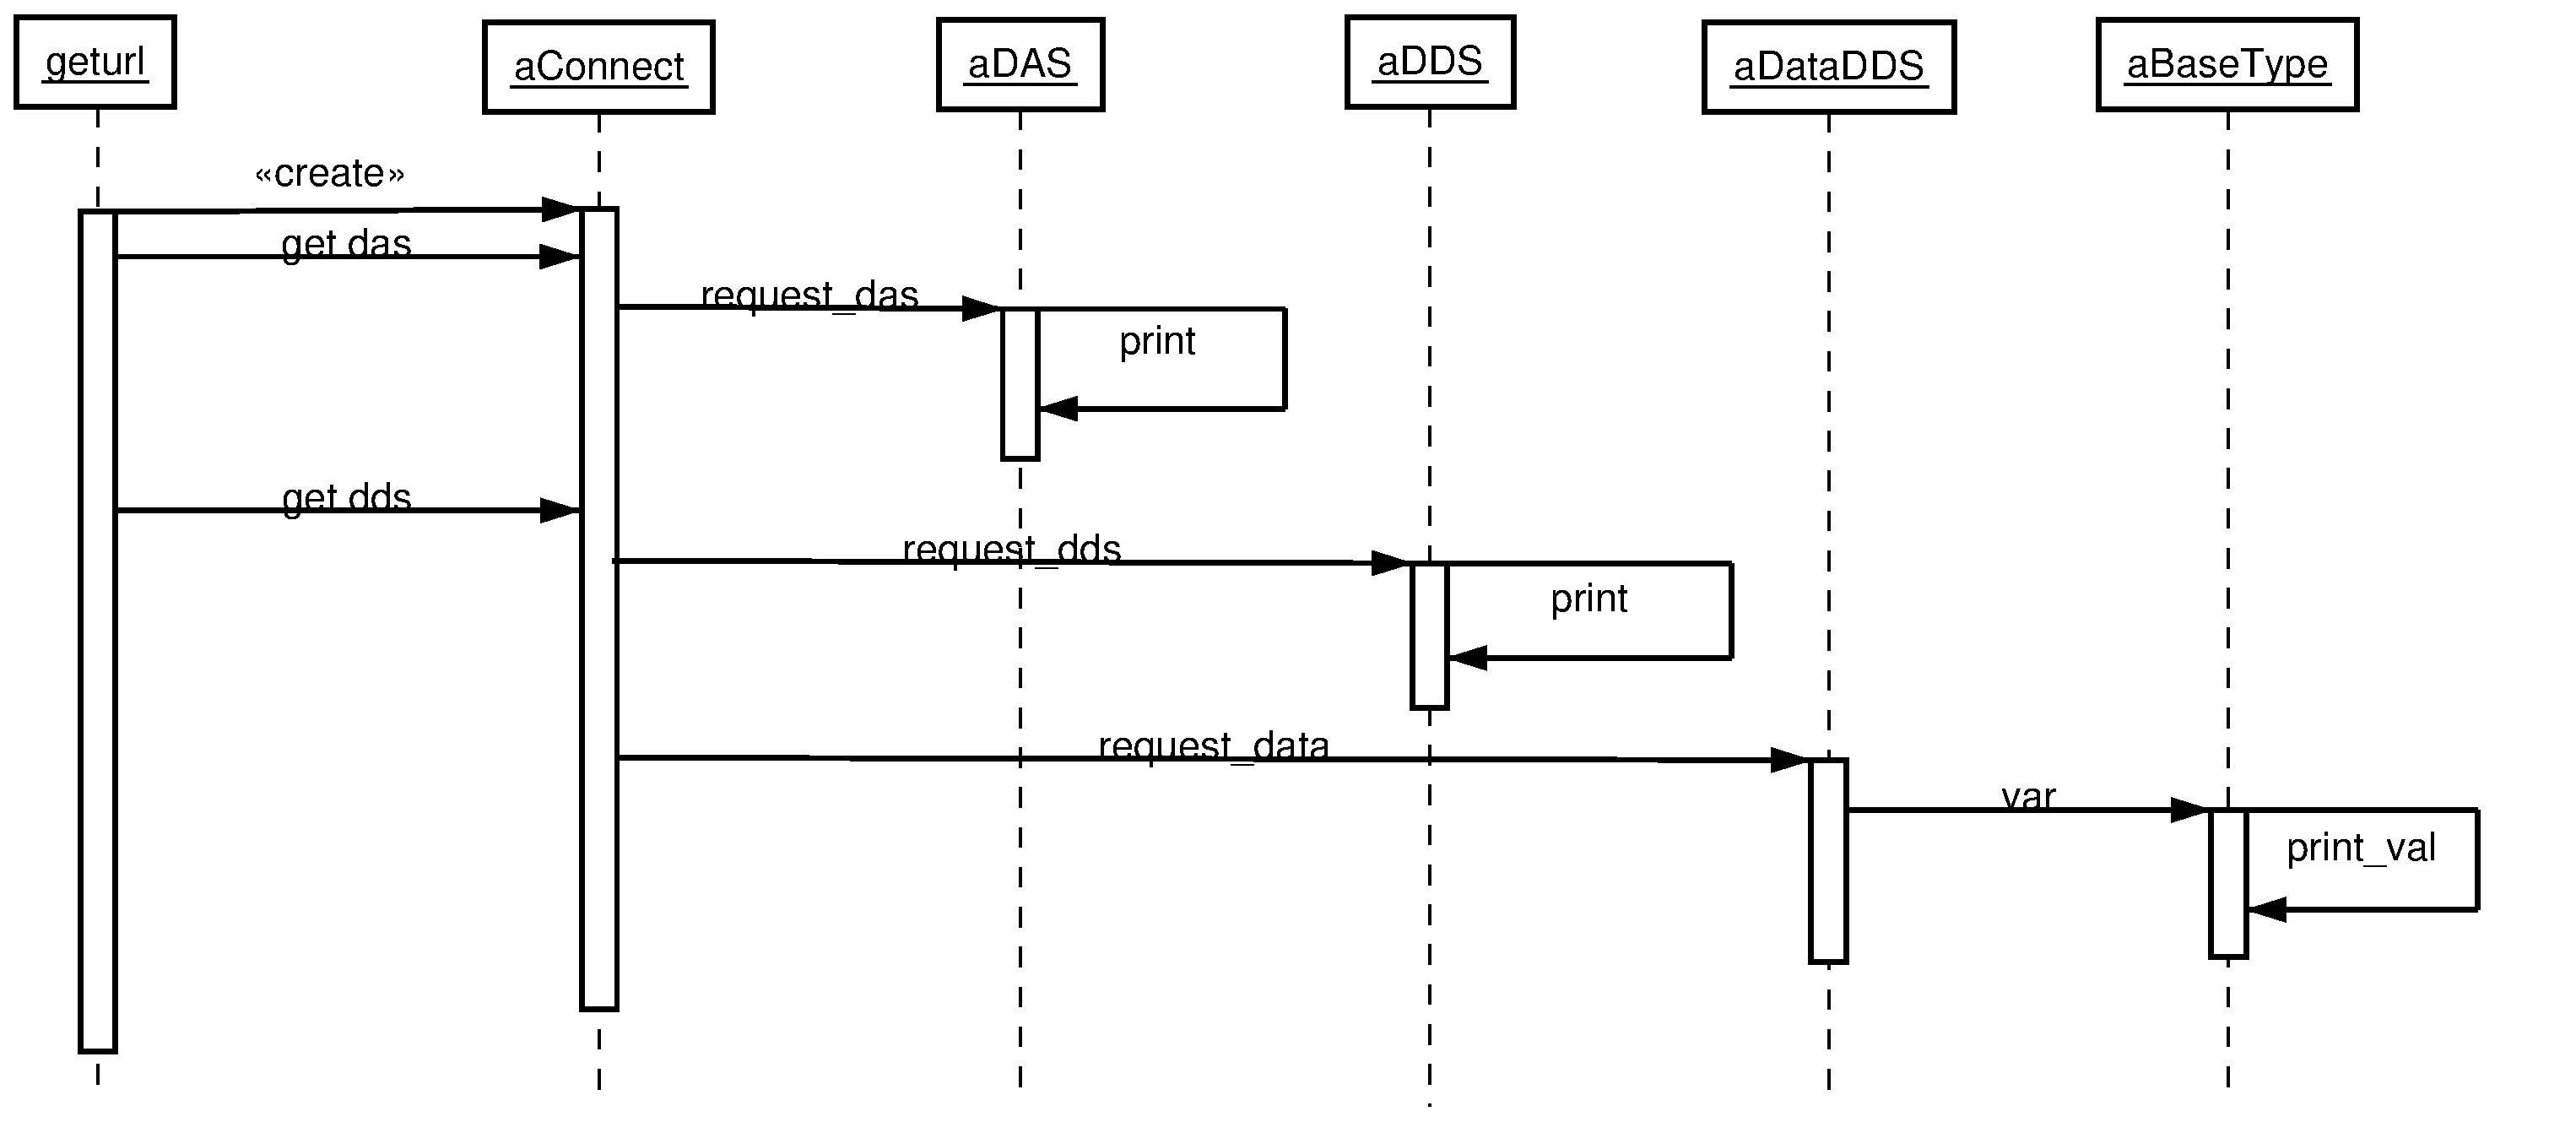
\epsfig{file=client-interaction.eps,width=7.5in}
\caption{Using the \dap class library to build a DODS client.}
\label{fig:client}
\end{center}
\end{sidewaysfigure}

% \clearpage
% \appendix

% \section{ChangeLog}
% \begin{verbatim}

% $Log: dap-description.tex,v $
% Revision 1.1  2000/11/07 04:00:36  jimg
% Created.
%
% Revision 1.2  2000/11/06 18:43:11  jimg
% Fixed grammar & spelling errors.
%
% Revision 1.1  2000/11/06 18:41:02  jimg
% First version.
%

% \end{verbatim}

\end{document}
